%!TEX root = ../thesis.tex
%*******************************************************************************
%*********************************** First Chapter *****************************
%*******************************************************************************

\chapter{Introduction}  %Title of the First Chapter

\ifpdf
    \graphicspath{{Chapter1/Figs/Raster/}{Chapter1/Figs/PDF/}{Chapter1/Figs/}}
\else
    \graphicspath{{Chapter1/Figs/Vector/}{Chapter1/Figs/}}
\fi

%********************************** % Section 1.1 **************************************
\section{Energy production and Sustainability\label{section1.1}}

Energy production is a critical aspect of modern societies, serving as the lifeblood for various activities that power economies, homes, and industries. Traditionally, energy production has relied heavily on fossil fuels such as coal, oil, and natural gas. However, the environmental impact and finite nature of these resources have led to a growing interest in alternative, sustainable sources of energy, giving rise to the concept of renewable energy.

\begin{figure}[htbp!] 
    \centering    
    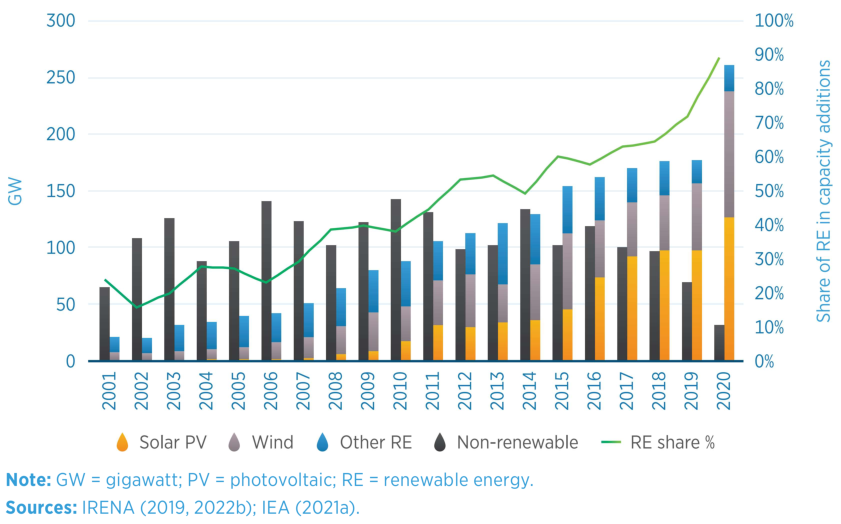
\includegraphics[width=0.8\textwidth]{01_fig_energy_production.pdf}
    \caption{IEA-ETSAP and IRENA© Technology Brief E06 – February 2015}
    \label{fig:production_energy_world}
\end{figure}

Renewable energy refers to energy derived from sources that are naturally restore on a human timescale. Unlike fossil fuels, which are finite and contribute to environmental degradation through greenhouse gas emissions, renewable energy sources are considered cleaner and more sustainable. Common types of renewable energy include solar power, wind power, hydropower, geothermal energy, and biomass. \dtd{lund2007}
Solar power harnesses the energy from the sun through photovoltaic cells, converting sunlight into electricity. Wind power utilizes the kinetic energy of the wind to turn turbines and generate electricity. Hydropower involves capturing the energy from moving water, often through dams or turbines. Geothermal energy taps into the Earth's internal heat for power generation. Biomass, on the other hand, involves converting organic materials such as plants and waste into energy.

The research of this thesis is focused on hydropower energy production. Hydropower stands as a well-established technology currently deployed in approximately 160 countries for the production of cost-effective, low-carbon, and renewable electricity. \dtd{irena}

Hydropower plants exhibit two fundamental configurations: those based on dams with reservoirs and run-of-the-river plants that lack reservoirs. Dams can further be classified into small dams with day-and-night regulation, large dams with seasonal storage, and pumped storage reversible plants capable of both generating and pumping for energy storage, adjusting to the fluctuations in electricity demand. Small-scale hydropower is frequently utilized for rural applications. \dtd{balmer}

With a cumulative capacity reaching around \SI{1060}{GW} (constituting \SI{19.4}{\%} of the world's electric capacity in 2011 \dtd{irena}), hydropower contributes to an annual electricity generation of about \SI{3500}{TWh}, accounting for \SI{15.8}{\%} of the global electricity generation in 2011. In over 35 countries, hydropower plants play a significant role by supplying at least \SI{50}{\%} of the total electricity demand. Italy is one of these countries with an installed capacity around \SI{19}{GW} hydropower plants generates about \SI{199}{TWh}, accounting for \SI{70}{\%} of the total electricity generation in 2022. \dtd{terna}

The optimization of hydropower energy production is one of the step forward the transition to renewable energy with the desire to reduce dependence on fossil fuels, and the recognition of the economic benefits associated with clean energy technologies. \dtd{barros, chun-thian} Governments and organizations worldwide are increasingly focusing on implementing policies and initiatives to promote the adoption of renewable energy and mitigate the impact of climate change.

Indeed, anticipating climate-change-induced changes in rainfall, water flows and extreme weather events is crucial for hydropower development planning as well as adequate power system planning. It is particularly important for governments, operators and decision makers to be aware of the issues that climate change can create on annual run-offs, their time distribution and sedimentation. The IHA produced a Climate Resilience Guide \dtd{Climate Resilience Guide} for the hydropower sector, which offers a methodology for identifying, assessing and managing climate risks to enhance the resilience of hydropower projects.

%% water-nexus means optimize the production maintaining the condition to use the water in other fields (agricultur irrigation) and protect the territories (flood control), and to satisfy the human uses and the quality of the water.

% digitalization
%% one of the main points to do it

%********************************** % Section 1.2 **************************************
\section{The Italian electricity market\label{section1.2}}

The electric market in Italy, established by the Legislative Decree of March 16, 1999, No. 79 (Legislative Decree No. 79/99), is a product of the transposition process of the European directive aiming to create an internal energy market (Directive 96/92/EC). This market is designed to address two specific needs: to promote competition in electricity production and trading and to ensure the economic management of dispatching services with criteria of neutrality, transparency, and objectivity.

The Italian electric market is divided into two main segments: the Spot Electricity Market (MPE) and the Forward Electricity Market (MTE). This research project is featured for the Spot Electricity Market, that further breaks down into the Day-Ahead Market (MGP), the Intraday Market (MI), the Daily Products Market (MPEG), and the Dispatching Service Market (MSD). The goal of the research in this thesis is based on the Day-Ahead Market (MGP).

The Day-Ahead Market (MGP) plays a crucial role in hosting the majority of electricity trading transactions. This market facilitates the exchange of hourly blocks of energy for the next day. The trading session opens at 8:00 am on the ninth day preceding the delivery day and closes at 12:00 pm on the day before the delivery day. The market results are communicated by 12:58 pm on the day before the delivery day.

Operators participate in the MGP by submitting bids that indicate the quantity and the maximum/minimum price at which they are willing to buy or sell electricity. The MGP operates as an auction market rather than a continuous trading market. Accepted bids are determined based on economic merit and within the limits of transit between zones.

The accepted purchase bids related to consumption units belonging to Italian geographical zones are valued at the National Single Price (PUN). The PUN is calculated as the average of the prices of geographical zones weighted by the quantities purchased in those zones. On the other hand, sale bids and purchase bids related to both pumping units and consumption units belonging to foreign virtual zones are valued at the marginal equilibrium price of the respective zones.

The GME (Electricity Market Operator) acts as the central counterparty, facilitating the trading activities in the market. The GME ensures the efficient functioning of the market by managing the acceptance of bids, determining equilibrium prices, and maintaining transparency and fairness in the trading process.

In summary, the Italian electric market, born out of legislative measures in 1999, operates with the aim of fostering competition and ensuring the economic management of dispatching services. The Spot Electricity Market, particularly the Day-Ahead Market, serves as a pivotal platform for electricity trading, with a focus on transparency, objectivity, and economic efficiency. The GME plays a central role in maintaining the integrity of the market, acting as a key intermediary in the trading activities between market participants.

%********************************** % Section 1.3 *************************************
\section{The challenges of this research\label{section1.3}}
% optimization for a sustainable energy production: prediction with confidence of the streamflow for the day-ahead market, with optimized use of the resources 
% digitalization of the meteo-hydro pipeline chain

%********************************** % Section 1.4 *************************************
\section{Region of Interest: the South Tyrol\label{section1.4}}

\subsection{Description of the area}
% description of the posizion, area and climatology
This research primarily concentrated on South Tyrol, a northern Italian Province. South Tyrol is an Alpine area distinguished by high elevation mountains separated by well defined valleys. The predominant geography of this region is influenced by three principal rivers: Adige, Isarco, and Rienza.

% main streams and lakes
The Adige River is the second-longest river in Italy and its catchment is the biggest in South Tyrol. Originating near the Reschen Pass, nestled in the Alps between Italy and Austria, this river courses through the western sector of the province until it reaches Bolzano. It collects here all water from the remaining South Tyrol region. Specifically, the Rienza River, originating at Braies Lake, traverses the Pusteria Valley and converges with the Isarco River near Bressanone. Subsequently, the Isarco River, with its source in the Brenner Pass, flows from north to south and merges with the Adige River in the town of Bolzano. From Bolzano to the hydrological closure of the Bolzano region all the remain water is collected in the Adige river.

In South Tyrol, there are approximately 350 lakes. All these bodies of water, whether in the mountains or on the plains, constitute extraordinary ecosystems that shape the landscape, host a wide variety of habitats for numerous animals and plants, and are therefore crucial for biodiversity conservation. Additionally, their presence adds value to the region as they serve as important recreational areas. The Province of Bolzano has always been committed to protecting this natural heritage and preserving the good quality of water, both chemically and ecologically.

The administrative area of South Tyrol is \SI{7400}{km^2} with elevation spanning from \SI{70}{\elevationunit} in Salorno to \SI{3950}{\elevationunit} of the Ortles peak. The case study climatology is well describes as Alpine, with precipitation and temperature as the main hydrological drivers. Average annual precipitation over the entire South Tyrol region is about \SI{1000}{mm}. In winter, the precipitation is partially retained as snowpack at the highest elevation where the temperature reaches \SI{-35}{\celsius} on the mountain peaks. The snow usually melts in spring and summer when the temperature rises with a maximum registered temperature of \SI{37}{\celsius} in Bolzano. On the other side, precipitation is concentrated mainly in summer and autumn with local and high-intensity storms. In these seasons, the combination of snow melting and higher precipitation event frequency leads to higher streamflow discharge in the rivers.

% population and demands
The population of South Tyrol is about 520000 inhabitants, with more than 200000 inhabitants located in the main cities of the region. The demand of water in this region is mainly divided in human use, agriculture and energy production. Water management in South Tyrol is crucial to ensuring a sustainable balance between water supply and demand. The local authorities through PGUAP and PTA monitor and implement measures to meet the needs of the population while maintaining the health of aquatic ecosystems and preserving water quality.

% energy production


\subsection{Data availability}
% ground stations
% Reanalysis data
% Forecast data
% Data Uncertainties

%********************************** % Section 1.5  *************************************
\section{Hydrological models and data-driven approach\label{section1.5}}  

\subsection{Hydrological models}
% hydrological models as forecaster, pros and cons
\subsection{Data-driven models}
% data-driven models as alternative..pros and cons


%********************************** % Section 1.6 *************************************
\section{Uncertainties propagation\label{section1.6}}  

\subsection{Weather Forecasting ensemble}
% ensemble as result of different initial condition
% ensemble as result of different models

\subsection{Data-driven hydrological ensemble}
% ensemble as result of different input data
% ensemble as result of different models

\subsection{Prediction confidence: uncertainty}
% definition of the confidence
% quantiles as confidence
% confidence as result of ensemble propagation